\documentclass{article}

\usepackage[utf8]{inputenc}
\usepackage{caption}
\usepackage{float}

\usepackage{tikz}
\usetikzlibrary{automata, positioning, arrows,
fit, % for the dashed boxes on Thompson's construction
calc
}

\newcommand{\emptystr}{\varepsilon}

\usepackage{hyperref}
\hypersetup{pdfauthor={Cristian Adrián Ontivero}}
\graphicspath{{imgs/}}

\newlength\tindent%
\setlength{\tindent}{\parindent}
\setlength{\parindent}{0pt}
\renewcommand{\indent}{\hspace*{\tindent}}

\renewcommand*{\tableautorefname}{Tabla}
\renewcommand*{\figureautorefname}{Figura}

%These tell TeX which packages to use.
\usepackage{array,epsfig}
\usepackage{amsmath}
\usepackage{amsfonts}
\usepackage{amssymb}
\usepackage{amsxtra}
\usepackage{amsthm}
\usepackage{mathrsfs}

%Here I define some theorem styles and shortcut commands for symbols I use often
\theoremstyle{definition}
\newtheorem{defn}{Definición}
\newtheorem{thm}{Teorema}
\newtheorem{cor}{Corolario}
\newtheorem*{rmk}{Remark}
\newtheorem{lem}{Lema}
\newtheorem*{joke}{Joke}

\newtheorem{ex}{Ejemplo}
\newcommand{\exautorefname}{Ejemplo}

\newtheorem{exercise}{Ejercicio}
\newcommand{\exerciseautorefname}{Ejercicio}

\newtheorem{soln}{Solución}
\newtheorem{prop}{Proposición}

\newcommand{\lra}{\longrightarrow}
\newcommand{\ra}{\rightarrow}
\newcommand{\surj}{\twoheadrightarrow}
\newcommand{\graph}{\mathrm{graph}}
\newcommand{\bb}[1]{\mathbb{#1}}
\newcommand{\Z}{\bb{Z}}
\newcommand{\Q}{\bb{Q}}
\newcommand{\R}{\bb{R}}
\newcommand{\C}{\bb{C}}
\newcommand{\N}{\bb{N}}
\newcommand{\M}{\mathbf{M}}
\newcommand{\m}{\mathbf{m}}
\newcommand{\MM}{\mathscr{M}}
\newcommand{\HH}{\mathscr{H}}
\newcommand{\Om}{\Omega}
\newcommand{\Ho}{\in\HH(\Om)}
\newcommand{\bd}{\partial}
\newcommand{\del}{\partial}
\newcommand{\bardel}{\overline\partial}
\newcommand{\textdf}[1]{\textbf{\textsf{#1}}\index{#1}}
\newcommand{\img}{\mathrm{img}}
\newcommand{\ip}[2]{\left\langle{#1},{#2}\right\rangle}
\newcommand{\inter}[1]{\mathrm{int}{#1}}
\newcommand{\exter}[1]{\mathrm{ext}{#1}}
\newcommand{\cl}[1]{\mathrm{cl}{#1}}
\newcommand{\ds}{\displaystyle}
\newcommand{\vol}{\mathrm{vol}}
\newcommand{\cnt}{\mathrm{ct}}
\newcommand{\osc}{\mathrm{osc}}
\newcommand{\LL}{\mathbf{L}}
\newcommand{\UU}{\mathbf{U}}
\newcommand{\support}{\mathrm{support}}
\newcommand{\AND}{\;\wedge\;}
\newcommand{\OR}{\;\vee\;}
\newcommand{\Oset}{\varnothing}
\newcommand{\st}{\ni}
\newcommand{\wh}{\widehat}

%Pagination stuff.
\setlength{\topmargin}{-.3 in}
\setlength{\oddsidemargin}{0in}
\setlength{\evensidemargin}{0in}
\setlength{\textheight}{9.in}
\setlength{\textwidth}{6.5in}
\pagestyle{empty}

\begin{document}

Brent's cycle detection algorithm \cite{Brent80}:

Brent's algorithm has a couple of advantages over Floyds: (1) for each step, it requires a
single evaluation of the next function instead of three; (2) Floyd's worst-case
complexity is an upper bound for Brent's, i.e. Brent's algorithm always requires the
same or less amount of steps; and (3) Brent's algorithm gives the cycle length
without requiring additional computation, while Floyd requires $\mathcal{O}(m)$
(TODO CHECK)
steps after detecting the loop. 

Improving on Floyd's cycle detection algorithm, the idea is having a fast
moving pointer (``hare''), and a stationary pointer (``turtle'') that jumps
(``teleports'') to the fast moving pointer's position whenever a certain
condition occurs. Doing this allows the fast pointer to get trapped in the cycle
fast, teleport the slow pointer to a node inside the loop, and keep moving the
fast pointer around the loop until it reaches the stationary pointer. 

\begin{figure}[ht] % ’ht’ tells LaTeX to place the figure ’here’ or at the top of the page
\centering % centers the figure
\begin{tikzpicture}[node distance=1cm,%
  every node/.style={fill, minimum size=2mm, inner sep=0pt, shape=circle, draw=black}
  ]
  \node[label=below:$x_1$] (x1) at (0,0) {};
  \node[label=below:$x_2$, right of=x1] (x2) {};
  \node[label=below:$x_m$, right=2cm of x2] (xm) {};
    \draw (x1) edge (x2);
    \draw (x2) edge[dashed] (xm);
  \end{tikzpicture}
\caption{Parity checker: accepts even Hamming weight strings.}
\label{fig:my_label}
\end{figure}

$\{x \in \Sigma^* \mid \text{the fifth symbol from the end of}~x~\text{is}~1 \} $

\begin{figure}[ht] % ’ht’ tells LaTeX to place the figure ’here’ or at the top of the page
\centering % centers the figure
\begin{tikzpicture}[node distance=2cm]
    \node[state, initial] (q0) {$q_0$};
    \node[state, right of=q0] (q1) {$q_1$};
    \node[state, right of=q1] (q2) {$q_2$};
    \node[state, right of=q2] (q3) {$q_3$};
    \node[state, right of=q3] (q4) {$q_4$};
    \node[state, right of=q4, accepting] (q5) {$q_5$};
    \draw (q0) edge node {1} (q1);
    \draw (q1) edge node {0,1} (q2);
    \draw (q2) edge node {0,1} (q3);
    \draw (q3) edge node {0,1} (q4);
    \draw (q4) edge node {0,1} (q5);
    \draw (q0) edge[loop above] node {0,1} (q0);
  \end{tikzpicture}
\caption{}
\label{fig:my_label}
\end{figure}

\begin{figure}[ht] % ’ht’ tells LaTeX to place the figure ’here’ or at the top of the page
\centering % centers the figure
\begin{tikzpicture}[node distance=2cm]
  \node[state, initial] (q0) {$q_0$};
    \node[state, right of=q0] (qa) {$q_a$};
    \node[state, right of=qa] (qaa) {$q_{aa}$};
    \node[state, accepting, right of=qaa] (qaaa) {$q_{aaa}$};
    \draw (q0) edge node {a} (qa);
    \draw (qa) edge node {a} (qaa);
    \draw (qaa) edge node {a} (qaaa);
    \draw (qaaa) edge[out=15, in=345, looseness=8] node {a} (qaaa);

  \node[state, initial, below of=q0] (q0') {$q_0'$};
    \node[state, right of=q0'] (qb) {$q_b$};
    \node[state, accepting, right of=qb] (qbb) {$q_{bb}$};
    \draw (q0') edge node {b} (qb);
    \draw (qb) edge node {b} (qbb);
    \draw (qbb) edge[out=15, in=345, looseness=8] node {b} (qbb);
\end{tikzpicture}
\caption{}
\label{fig:m1-m2}
\end{figure}

\begin{figure}[ht] % ’ht’ tells LaTeX to place the figure ’here’ or at the top of the page
\centering % centers the figure
\begin{tikzpicture}[node distance=2.6cm, every state/.style={thick, minimum
  size=46pt, font=\footnotesize}]
  \node[state, initial] (q0q0') at (0,0) {$(q_0,q_0')$};
    \node[state, right of=q0q0'] (qaq0') {$(q_a, q_0')$};
    \node[state, right of=qaq0'] (qaaq0') {$(q_{aa}, q_0')$};
    \node[state, right of=qaaq0'] (qaaaq0') {$(q_{aaa}, q_0')$};
    \draw (q0q0') edge node {a} (qaq0');
    \draw (qaq0') edge node {a} (qaaq0');
    \draw (qaaq0') edge node {a} (qaaaq0');


    \node[state, below of=q0q0'] (q0qb) {$(q_0, q_b)$};
    \node[state, right of=q0qb] (qaqb) {$(q_a, q_b)$};
    \node[state, right of=qaqb] (qaaqb) {$(q_{aa}, q_b)$};
    \node[state, right of=qaaqb] (qaaaqb) {$(q_{aaa}, q_b)$};
    \draw (q0qb) edge node {a} (qaqb);
    \draw (qaqb) edge node {a} (qaaqb);
    \draw (qaaqb) edge node {a} (qaaaqb);

    \node[state, below of=q0qb] (q0qbb) {$(q_0, q_{bb})$};
    \node[state, right of=q0qbb] (qaqbb) {$(q_a, q_{bb})$};
    \node[state, right of=qaqbb] (qaaqbb) {$(q_{aa}, q_{bb})$};
    \node[state, accepting, right of=qaaqbb] (qaaaqbb) {$(q_{aaa}, q_{bb})$};
    \draw (q0qbb) edge node {a} (qaqbb);
    \draw (qaqbb) edge node {a} (qaaqbb);
    \draw (qaaqbb) edge node {a} (qaaaqbb);

    \draw (q0q0') edge node {b} (q0qb);
    \draw (q0qb) edge node {b} (q0qbb);
    \draw (qaq0') edge node {b} (qaqb);
    \draw (qaqb) edge node {b} (qaqbb);
    \draw (qaaq0') edge node {b} (qaaqb);
    \draw (qaaqb) edge node {b} (qaaqbb);
    \draw (qaaaq0') edge node {b} (qaaaqb);
    \draw (qaaaqb) edge node {b} (qaaaqbb);
    \draw (qaaaq0') edge[out=15, in=345, looseness=8] node {a} (qaaaq0');
    \draw (qaaaqb) edge[out=15, in=345, looseness=8] node {a} (qaaaqb);
    \draw (qaaaqbb) edge[out=15, in=345, looseness=8] node {a,b} (qaaaqbb);

    \draw[out=255, in=285, looseness=6] (q0qbb) edge node[below] {b} (q0qbb);
    \draw[out=255, in=285, looseness=6] (qaqbb) edge node[below] {b} (qaqbb);
    \draw[out=255, in=285, looseness=6] (qaaqbb) edge node[below] {b} (qaaqbb);
    \draw[out=255, in=285, looseness=6] (qaaaqbb) edge node[below] {b} (qaaaqbb);

  \end{tikzpicture}
\caption{}
\label{fig:m3}
\end{figure}

\newpage 
\bibliography{refs}
\bibliographystyle{unsrt}

\end{document}


